\let\counterwithout\relax
\let\counterwithin\relax
\documentclass[final]{fhnwreport}       %[mode] = draft or final
\usepackage{color, colortbl}
\usepackage{rotating, rotfloat,ragged2e, hyphenat, diagbox, wrapfig}
\definecolor{grau}{gray}{0.9}
\definecolor{hellgrau}{gray}{0.95}

                                        %{class} = fhnwreport, article, 
                                        %          report, book, beamer, standalone
%%---Main Packages-----------------------------------------------------------------------
\usepackage[english, ngerman]{babel}	%Mul­tilin­gual sup­port for LaTeX
\usepackage[T1]{fontenc}				%Stan­dard pack­age for se­lect­ing font en­cod­ings
\usepackage[utf8]{inputenc}				%Ac­cept dif­fer­ent in­put en­cod­ings
\usepackage{lmodern}                    %The newer Font-Set
\usepackage{textcomp}					%LaTeX sup­port for the Text Com­pan­ion fonts
\usepackage{graphicx} 					%En­hanced sup­port for graph­ics
\usepackage{float}						%Im­proved in­ter­face for float­ing ob­jects
\usepackage{ifdraft}                    %Let you check if the doc is in draft mode

%%---Useful Packages---------------------------------------------------------------------
\usepackage[pdftex,dvipsnames]{xcolor}  %Driver-in­de­pen­dent color ex­ten­sions for LaTeX
\usepackage{csquotes}                   %Simpler quoting with \enquote{}
\usepackage{siunitx} 					%A com­pre­hen­sive (SI) units pack­age
\usepackage{listings}					%Type­set source code list­ings us­ing LaTeX
\usepackage[bottom]{footmisc}			%A range of foot­note op­tions
\usepackage{footnote}					%Im­prove on LaTeX's foot­note han­dling
\usepackage{verbatim}					%Reim­ple­men­ta­tion of and ex­ten­sions to LaTeX ver­ba­tim
\usepackage[textsize=footnotesize]{todonotes} %Mark­ing things to do in a LaTeX doc­u­ment

%%---Tikz Packages-----------------------------------------------------------------------
\usepackage{standalone}
\usepackage{tikz}
\usepackage{circuitikz}
\usetikzlibrary{arrows}
\usetikzlibrary{calc}
\usetikzlibrary{intersections}

%%---Math Packages-----------------------------------------------------------------------
\usepackage{amsmath}					%AMS math­e­mat­i­cal fa­cil­i­ties for LaTeX
%\usepackage{amssymb}					%Type­set­ting symbols (AMS style)
%\usepackage{array}						%Ex­tend­ing the ar­ray and tab­u­lar en­vi­ron­ments
%\usepackage{amsthm}					%Type­set­ting the­o­rems (AMS style)

%%---Table Packages----------------------------------------------------------------------
\usepackage{tabularx}					%Tab­u­lars with ad­justable-width columns
%\usepackage{longtable}
\usepackage{multirow}					%Create tab­u­lar cells span­ning mul­ti­ple rows
\usepackage{multicol}					%In­ter­mix sin­gle and mul­ti­ple columns

%%---PDF / Figure Packages---------------------------------------------------------------
\usepackage{pdfpages}					%In­clude PDF doc­u­ments in LaTeX
\usepackage{pdflscape}					%Make land­scape pages dis­play as land­scape
\usepackage{subfig}					    %Fig­ures di­vided into sub­fig­ures

%%---Other Packages----------------------------------------------------------------------
%\usepackage{xargs}                     %De­fine com­mands with many op­tional ar­gu­ments

%%---Bibliography------------------------------------------------------------------------
\usepackage[style=ieee,urldate=comp,backend=biber]{biblatex}
\addbibresource{literature/bibliography.bib}

%%---Main Settings-----------------------------------------------------------------------
\graphicspath{{./graphics/}}			%Defines the graphicspath
%\geometry{twoside=false}				    %twoside=false disables the "bookstyle"
\setlength{\marginparwidth}{2cm}
\overfullrule=5em						%Creates a black rule if text goes over the margins => debugging


%%---User Definitions--------------------------------------------------------------------
%%Tabel-Definitions: (requires \usepackage{tabularx})
\newcolumntype{L}[1]{>{\raggedright\arraybackslash}p{#1}}    %column-width and alignment
\newcolumntype{C}[1]{>{\centering\arraybackslash}p{#1}}
\newcolumntype{R}[1]{>{\raggedleft\arraybackslash}p{#1}}

%%---Optional Package Settings-----------------------------------------------------------
%Listings-Settings: (requires \usepackage{listings}) => Example with Matlab Code
\lstset{language=Matlab,%
    basicstyle=\footnotesize\ttfamily,
    breaklines=false,%
    morekeywords={switch, case, otherwise},
    keywordstyle=\color{Blue},%
    tabsize=2,
    %morekeywords=[2]{1}, keywordstyle=[2]{\color{black}},
    identifierstyle=\color{Black},%
    stringstyle=\color{Purple},
    commentstyle=\color{Green},%
    showstringspaces=false,%without this there will be a symbol in the places where there is a space
    numbers=left,%
    numberstyle={\tiny \color{black}},% size of the numbers
    numbersep=9pt, % this defines how far the numbers are from the text
    %emph=[1]{word1, word2,...},emphstyle=[1]\color{red}
}							
			                %loads all packages, definitions and settings												
\title{«DJ» EMI Filter für Schaltnetzteil}          			%Project Title
\author{Pflichtenheft technischer Teil}  		%Document Type => Technical Report, ...
\date{Windisch, 04.04.2019}             		%Place and Date

\begin{document}

%%---TITLEPAGE---------------------------------------------------------------------------
\selectlanguage{ngerman}                %ngerman or english
\maketitle

\vspace*{-1cm}						    %compensates the space after the date line.
\vfill
\begin{figure}[H]
\centering
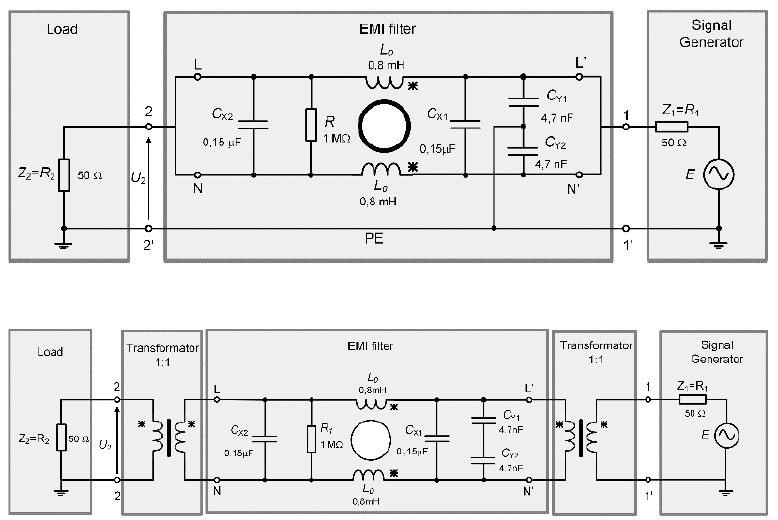
\includegraphics[width=10cm]{titelBild.png}
\end{figure}
\vfill

{
\renewcommand\arraystretch{2}
\begin{center}
\begin{tabular}{ >{\bf} l p{10cm} l }
Hochschule&Hochschule für Technik - FHNW\\
Studiengang&Elektro- und Informationstechnik\\
Auftraggeber&Dr. Luca Dalessandro\\
Betreuer&Prof. Dr. Sebastian Gaulocher \newline Prof. Peter Niklaus \newline Prof. Dr. Richard Gut \newline  Dr. Anita Gertiser \newline Pascal Buchschacher \\
Autoren&\textbf{Gruppe 1} \newline Niklaus Schwegler \newline Lukas von Däniken \newline Pascal Puschmann \newline Alfare Claudio \newline Simon Rohrer \\
Version&1.0 %Normally not used!
\end{tabular}
\end{center}
}

\clearpage

%\selectlanguage{ngerman}				%ngerman or english
\thispagestyle{empty}
			
%%---TABLE OF CONTENTS-------------------------------------------------------------------
\pagenumbering{Roman}		
%\selectlanguage{ngerman}				%ngerman or english
\tableofcontents
\clearpage

%%---TEXT--------------------------------------------------------------------------------
\pagenumbering{arabic}
\section{Übersicht} \label{sec:uebersicht}
\subsection{Ausgangslage}

In der modernen Gesellschaft hängen von Jahr zu Jahr mehr elektrische Verbraucher am Stromnetz. Der stetig steigende Leistungsbedarf dieser Verbraucher führt dazu, dass ihre Versorgung angepasst werden muss. Aus dem konventionellen Trafo-Netzteil entstand das sogenannte Schaltnetzteil. Dieses hat grosse Vorteile gegenüber dem Trafo-Netzteil, sowohl wirtschaftlich gesehen, als auch leistungsbezogen. \\Allerdings haben sie auch einen Nachteil. Sie lassen hochfrequente Störungen (EMI), entstehen, welche ins Netz zurückfliessen. Diese Störungen, welche man als Gleichtakt- und Gegentaktrauschen bezeichnet, können wiederum in anderen Verbrauchern  Störungen verursachen. \\Aufgrund dieses Problems wurden verschiedene Normen an Geräte gestellt um diese Emissionen zu minimieren. Daher werden in moderne Schaltnetzteile EMI-Filter verbaut.  Diese, auch Netzfilter genannt, bestehen aus einem Netzwerk von  aus Widerständen, Kondensatoren und Spulen. Da im Schaltnetzteil die Netzfrequenz in eine hochfrequente Spannung gewandlet wird, reagieren die Bauteile als Impedanzen und sie filtern, je nach Bauform, verschiedene hochfrequente Signale aus der Rückspeisung.


Der Auftrag von Dr. Dalessandro lautet eine Applikation zu entwickeln, welche in der Entwicklung von solchen Filtern eingesetzt werden kann. Die Anforderungen an die Applikation sind, dass die Dämpfungseigenschaften des Filters simuliert und graphisch angezeigt werden können. Dabei sollen die Gleichtakt- und die Gegentaktstörungen differenziert betrachtet weden können. Ebenfalls soll die Applikation in der Lage sein, die parasitären Einflüsse der einzelnen Parameter (Bauteile) um ± 30 \% zu variieren.   


Dieses Pflichtenheft beschreibt die technischen Aspekte des Auftrags und liefert bereits Ideen betreffend der Umsetzung. 
 

\newpage
\subsection{Projektziele} \label{subsec:projektziele}


In der Folgenden Tabelle werden alle Ziele aufgeleistet. In Kapitel 2 werden sie ausformuliert und ihre Implementation wird erläutert. 
\newcommand{\HY}{\hyphenpenalty = 25\exhyphenpenalty = 25}
\begin{table}[H]
\small
\begin{tabular}{>{\HY\RaggedRight}p{7cm} >{\HY\RaggedRight}p{1.5cm} >{\HY\RaggedRight}p{1.5cm} >{\HY\RaggedRight}p{3cm}}
\hline
\textbf{Ziel}					&\textbf{Muss}	&\textbf{Soll}	&\textbf{Zielbezeichnung}			\\						
\hline
\rowcolor{hellgrau}
\multicolumn{4}{l}{\textbf{Fachliche Anforderung}}\\
Unabhängigkeit von Betriebssystemen		&\ x &\  &\ F1\\
Modular aufgebaut/erweiterbar		&\ x &\  &\ F2\\
Berechnungen und GUI getrennt		&\ x &\  &\ F3\\
 Berechnungszeit < 10 Sek.		&\ x &\  &\ F4\\
Unabhängige Komponenten		&\   &\ x &\ F5\\
Verstellbare Parameter		&\ x &\   &\ F6\\
Verschiedene Berechnungsmodi		&\ x &\   &\ F7\\	
Monte-Carlo Simulation &\   &\ x &\ F8\\

\rowcolor{hellgrau}
\multicolumn{4}{l}{\textbf{Graphische Anforderungen}}\\			
Visualisierung der Schaltung		&\  &\ x &\ G1\\	
Einfache und schnelle Eingabemöglichkeit &\ x &\  &\ G2\\
Darstellung im Frequenzbereich bis 30MHz		&\ x &\  &\ G3\\
Mehrere Plots gleichzeitig		&\ x &\  &\ G4\\
Auslagern des Plots		&\   &\ x &\ G5\\


\rowcolor{hellgrau}
\multicolumn{4}{l}{\textbf{Anforderungen an die Bedienung}}\\			
Schutz vor Fehleingaben		&\ x &\   &\ B1\\
Export von Plots		&\  &\ x &\ B2\\
Speicherverwaltung		&\   &\ x &\ B3\\
Import von Daten		&\   &\ x &\ B4\\	
				
\hline
\end{tabular}
\end{table}

\newpage
\subsection{Lieferobjekte} \label{subsec:lieferobjekt}

Nachfolgend werden alle Lieferobjekte aufgelistet:

\newcommand{\HE}{\hyphenpenalty = 25\exhyphenpenalty = 25}
\begin{table}[H]\label{tab:lieferobjekte}
\small
\begin{tabular}{>{\HE\RaggedRight}p{5.5cm} >{\HE\RaggedRight}p{4cm} }
\hline
\rowcolor{hellgrau}
\textbf{Beschreibung}					&\textbf{Datum}			\\						
\hline
%\rowcolor{hellgrau}
%\multicolumn{2}{l}{\textbf{Objekt} } {\textbf{Datum}}\\
1. Organisatorisches Pflichtenheft		&\ 24.03.19 und 04.04.19\\
2. Technisches Pflichtenheft		&\ 24.03.19 und 04.04.19\\
3. Beta-Version des GUI	&\ 18.04.19\\
4. Beta-Version der Software &\ 28.04.19\\
5. Fachbericht	&\ 13.06.19\\
\hline
\end{tabular}
\end{table}

\section{Theoretische Grundlagen} \label{sec:TheoretischeGrundlagen}

\subsection{EMI-Filter} \label{subsec:emifilter}
Das vorgegebene EMI-Filter muss bezüglich der Einfügungsverluste (insertion loss) untersucht werden. Die Einfügunsverluste hängen vom Gesamtrauschen der Schaltung ab. Es wird ein Ansatz verwendet der in der Praxis weit verbreitet ist, bei welchem das Gesamtrauschen in zwei Komponenten unterteilt wird. Man spricht vom Gegen-(=Differential Mode=DM) und Gleichtaktrauschen (=Common Mode=CM) . Anhand der vorgegebenen CM- und DM-Äquivalenten Schaltungen werden die Einfügungsverluste in Funktion der Frequenz berechnet. Die Berechnungen decken einen Bereich von 0 bis 30MHz ab.

Die Einfügungsverluste sind wie folgt definiert: 

\begin{figure}[H]
	\centering
	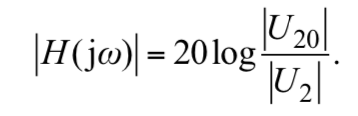
\includegraphics[width=5cm]{def_insertionloss.png}
	\caption{insertionloss}
	\label{fig:insertion loss}
\end{figure}
Wobei H dem Streuparameter (S-Parameter) S index 21 entspricht. Die Einfügungsverluste sind auch mit dem Verhältnis von eingehenden zu abegegebenen Leistung zu Berechnen, jedoch eignet sich diese Methode mehr beim messtechnischen bestimmen der Einfügungsverluste. Da die Berechnungen in einem Bereich von bis zu 30 MHz gemacht werden, ist es notwendig die parasitären Parameter von Spule und Kondensator miteinzubeziehen. Zudem können sie in einem Bereich von +- 30% vaariert werden.

\subsection{Schaltungen} \label{subsec:schaltungen}
CM:
\begin{figure}[H]
	\centering
	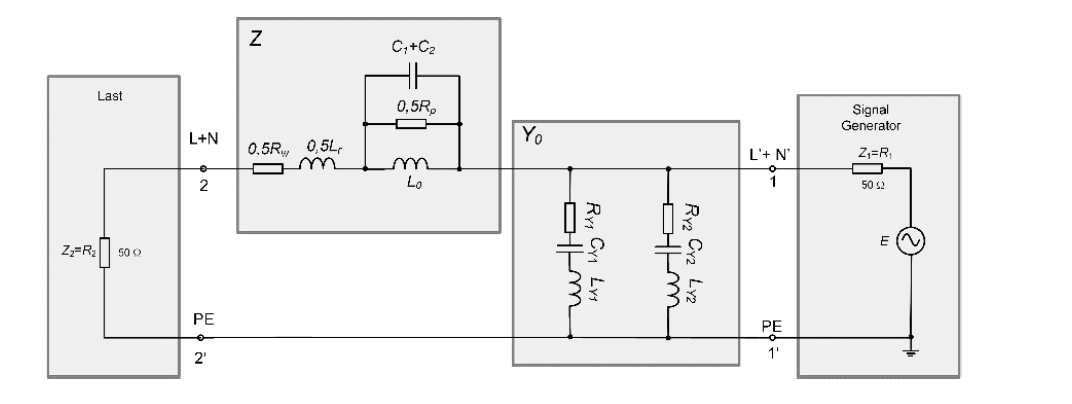
\includegraphics[width=15cm]{CM_ElectricalCircuit.png}
	\caption{CM-Schaltungäquvalent}
	\label{fig:CM-Schaltungäquvalent}
\end{figure}
DM:
\begin{figure}[H]
	\centering
	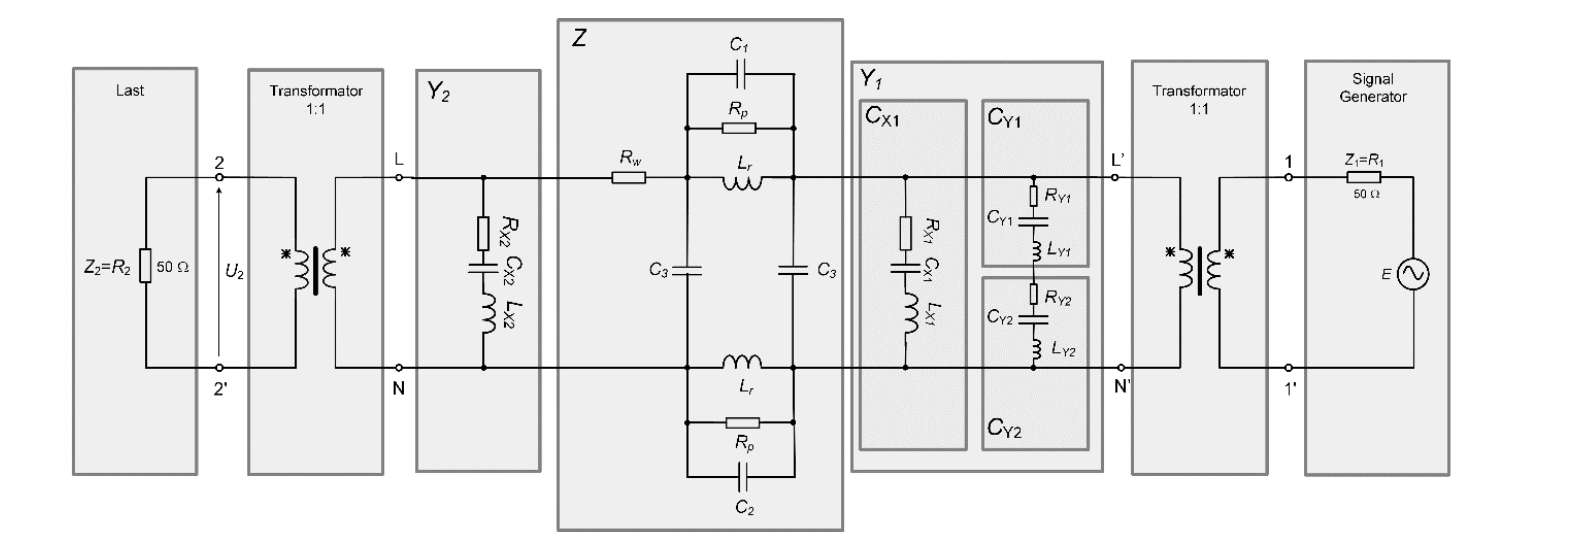
\includegraphics[width=15cm]{DM_ElectricalCircuit.png}
	\caption{DM-Schaltungsäquvalent}
	\label{fig:DM-Schaltungsäquvalent}
\end{figure}
\subsection{Vorgehen} \label{subsec:vorgehen}
Die Einfügungsverluste werden analytisch ermittelt. Im ersten Schritt werden die Berechnungen in MATLAB gemacht. Somit können die Funktionen eifach geplottet werden. Diese Plots werden dann mit Simulationen in MPLAB Mindi verglichen um festzustellen ob diese korrekt sind. Die vollständigen und korrekten Berechnungen können somit in Java implementiert werden. Um die Einfügungsverluste bestimmen zu können, wird das Model der 2-Tore verwendet. Einzelne Schaltungsteile werden in ABCD-Matrixen abgebildet, welche dann durch Kaskadierung der einzelnen ABCD-Matrixen zusammengeführt werden. Die Einfügungsverluste werden den S-Parameter abgeleitet, welche direkt aus der ABCD-Matrix errechnet werden kann.
Der S-Parameter Index 12 gibt den Tranmissionsgrad der Wellen an, die vom Tor 1 zum Tor2 übertragen wird. Die S-Parameter sind abhängig von den Bezugswiderständen (Innenwiderstand der Quelle sowie Lastwiderstand). In unserem Fall sind die Bezugswiderstände mit 50Ohm gegeben.

\newpage
\subsection{Beispiel} \label{subsec:beispiel}

\begin{equation}
IL= -20*log(\left\lvert S_{21} \right\rvert)
\end{equation}
Bei der Definition der Einfügungsverluste kann für das Verhältnis der Spannungen der Streuparameter S21 eingesetzt werden. Der Streuparameter wird wie folgt berechnet.
Schritt1: Berechnen der Längsimpedanz Z und der Queradmittanz Y0.
Für die Querimpedanz Y0 ergibt sich die Formel
\begin{equation}
Y_0 = \frac{ 1 }{R_{y1} + \frac{1}{j*\omega*C_{y1}}+j*\omega*L_{y1}} +\frac{ 1 }{R_{y2} + \frac{1}{j*\omega*C_{y2}}+j*\omega*L_{y2}}
\end{equation}
\begin{figure}[H]
	\centering
	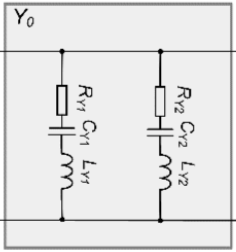
\includegraphics[width=5cm]{CM_Admittanz.png}
	\caption{CM-Admittanz}
	\label{fig:CM-Admittanz}
\end{figure}
Für die Impedanz Z ergibt sich folgende Formel
\begin{equation}
Z = 0.5*R_w+j*\omega*L_r+\frac{ 1 }{ \frac{1}{0.5*R_p}+j*\omega*L_r*(C_1+C_2)+\frac{1}{j*\omega*L_0} }
\end{equation}

\begin{figure}[H]
	\centering
	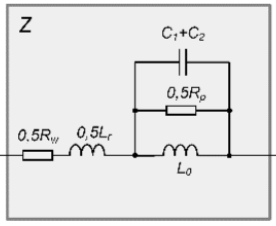
\includegraphics[width=5cm]{CM_Impedanz.png}
	\caption{CM-Impedanz}
	\label{fig:CM-Impedanz}
\end{figure}
Schritt2: Erstellen der ABCD-Matrixen.

Somit ergeben sich die ABCD-Matrixen wie folgt
\begin{equation}
A_1 =
\begin{matrix}
1 & 0\\ Y&1 
\end{matrix}
\end{equation}
\begin{equation}
A_2 =
\begin{matrix}
1 & Z\\ 0&1 
\end{matrix}
\end{equation}


Die ABCD-Matrixen haben den Vorteil, dass man sie sehr unkompliziert kaskadieren kann indem man das Produkt bildet.
\begin{equation}
A = A_1*A_2
\end{equation}

Schritt3: S21 Parameter bilden.

Der S21 Parameter ist wie folgt definiert.

\begin{equation}
S_{21} = \frac{2}{A_{11}+\frac{A{12}}{R_w}+A_{21}*R_w+A_{22}}
\end{equation}

Somit sind alle gesuchten Werte gegeben und der S21 Parameter wird durch einsetzen der Werte gebildet.

Schritt4: Einfügungsverluste bilden

Durch Einsetzen des Streuparameters S21 in die Definition der Einfügunsverluste, lassen sich diese Darstellen. Folgende Grafik zeigt die Berechnungen in MATLAB. 


\begin{figure}[H]
	\centering
	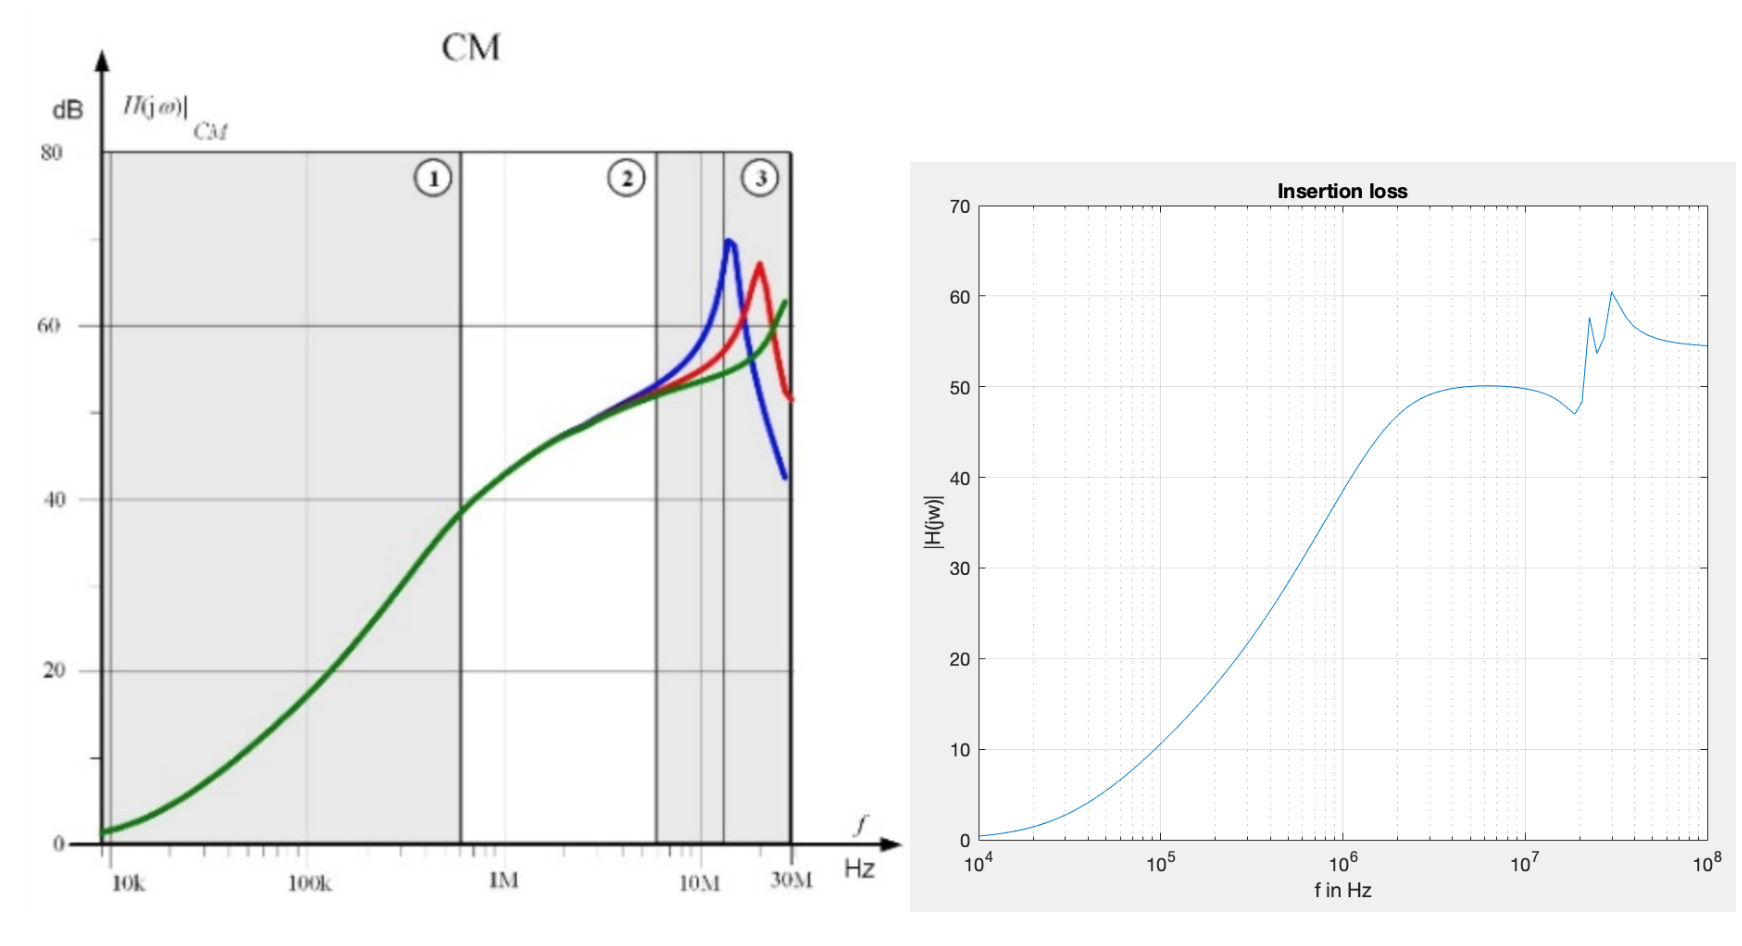
\includegraphics[width=15cm]{CM_vergleich.png}
	\caption{Vergleich}
	\label{fig:Vergleich Berechnung Simulation}
\end{figure}

\section{Softwarekonzept} \label{sec:softwarekonzept}

Um das sämtliche Anforderungen an die Software zu erfüllen wurden alle Probleme erfasst und in Teilprobleme aufgeteilt. Angefangen von der Grundstruktur der Software werden wir von Oben herab, sogenannt Top-Down, jeweils Lösungen für die einzelnen Teilprobleme erarbeiten. Durch die MVC-Grundstruktur können all diese Teilprobleme unabhängig von einander behandelt werden. Dies erlaubt eine kluge und effiziente Arbeitsaufteilung.

Die Beschreibung des Softwarekonzepts wird in 2 Sektionen unterteilt. Zuerst werden die in der Zieltabelle aufgeführten technischen und die graphischen Anforderungen beschrieben.  Anschliessend werden die Anforderungen an die Bedienung definiert. und zum Schluss werden die einzelnen Elemente der GUI, und somit die Bedienung erklärt.

\subsection{Programmablauf} \label{subsec:programmablauf}

Der folgende Programmablauf ist auf die Maximallösung bezogen. In dieser Lösung sind alle Wunschziele (Kapitel: \ref{subsec:projektziele}) vorhanden.

Nach dem Aufstarten des Programmes kann der Benutzer über die Programmoberfläche (Abbildung: \ref{fig:GUI}) seine Simulationen starten.
Am Anfang ist ein default Filter initialisiert. Dieser ist in der Filtertabelle eingetragen, jedoch sind die parasitären Filterparameter im Eingabefenster noch undefiniert. Der Benutzer kann diese nun definieren und die berechneten Einfügungsverluste von CM und DM des EMI-Filters werden im Plot dargestellt. Mit dem Button Add wird der Filter abgespeichert und ein neuer Filter kann definiert werden. Es können somit mehrere Filter gleichzeitig dargestellt werden. 

Um die Filter richtig zu verwalten ist es möglich in der Filtertabelle über die Checkbox einzelne Filter im Plot ein und auszublenden. Ebenfalls können sie spezifisch benannt werden. Der Plot und die einzelnen Kurven können mit einem Rechtsklick auf den CM/DM Plot individuell angepasst und auch exportiert werde. Wird ein Filter nicht mehr benötigt kann er in der Filtertabelle angewählt und mit dem Button Remove entfernt werden. Damit der Benutzer nicht jedesmal die Filterprofile einstellen muss, können diese über File/Save filterprofil in einer .txt Datei abgespeichert werden. Bei einem Neustart des Programmes können über File/Load filterprofile die Filterprofile wieder geladen werden. 

Um die Auswirkungen einzelner parasitären Filterparameter besser zu analysieren, kann unter Simulation/Monte Carlo eine Monte Carlo Simulation gestartet werden. Es wird ein neues Fenster geöffnet in dem der Filterparameter, die Toleranz und die Anzahl Berechnungen eingestellt werden können. Jede Berechnung wird als einzelner Filter in die Filtertabelle geladen. Um nachzuschauen wo welche Filterparameter sich in der Schaltung befinden, können unter Help/CM electrical circuit und CM electrical circuit die Ersatzschaltungen, von der die Berechnungen ausgehen, angeschaut werden. Das Programm wird über File/Exit oder beim Schliessen des Fensters beendet.

Das Klassendiagramm der Software ist in der Abbildung \ref{fig:Klassendiagramm} ersichtlich.

\newpage

\subsubsection{Klassendiagramm} \label{subsubsec:Klassendiagramm}

\begin{figure}[H]
	\centering
	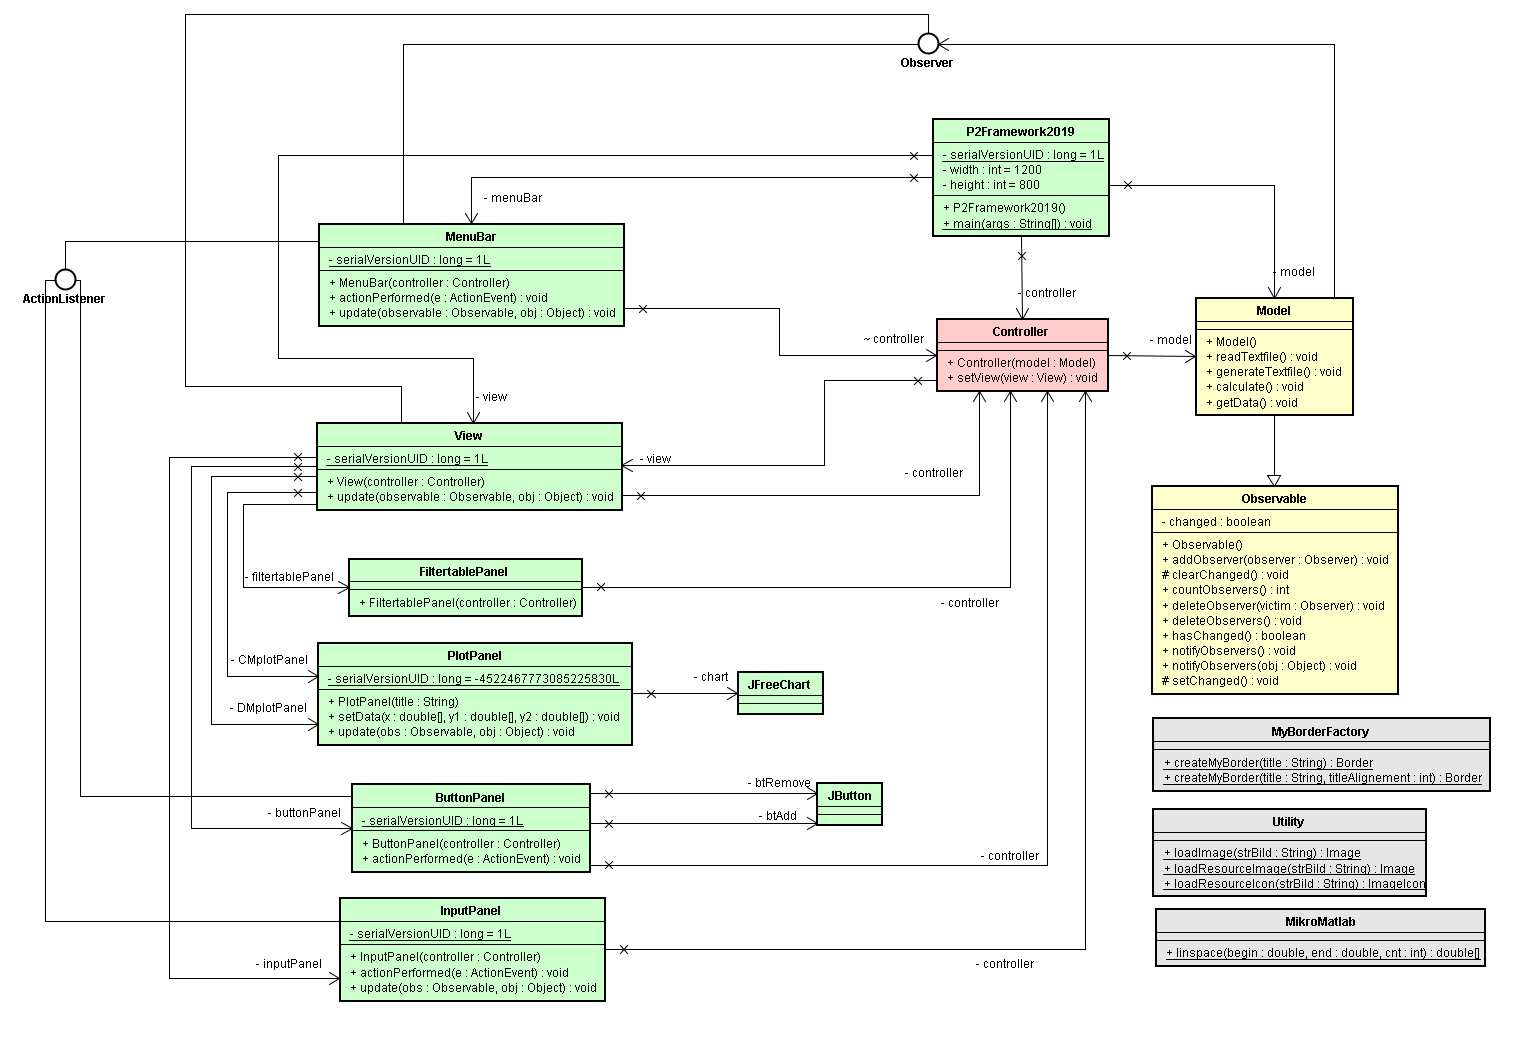
\includegraphics[width=16cm]{Klassendiagramm.png}
	\caption{Klassendiagramm}
	\label{fig:Klassendiagramm}
\end{figure} 

\newpage

\subsection{Analytische Anforderungen} \label{subsubsec:analytischeanforderungen}

\bigskip
\shorthandoff{"}
\subsubsection{Softwarestruktur} \label{subsubsec:Softwarestruktur}
Die Software ist mit Java geschrieben und ist somit Plattformunabhängig. Die Software wird mit dem Model-View-Controller Entwurfsmuster (MVC Design Pattern) \cite{MVCDesignPattern} strukturiert. Durch diese Strukturierung ist es weitgehend möglich die Daten und deren graphische Repräsentation zu trennen. Dies vereinfacht Wartungsarbeiten und die Wiederverwendbarkeit von Programmteilen. Die Struktur ist in die drei Teile: Modell (engl. model), Präsentation (engl. view) und Steuerung (engl. controller) unterteilt.

\bigskip
\subsubsection{Mathematische Anforderungen}\label{subsubsec:mathematischeanforderungen}
Das elektrische Verhalten der CM- und DM-äquivalenten Schaltungen, wird anhand der Streuparameter $S_{21}$ beschrieben. Um den Streuparameter $S_{21}$ zu bestimmen, werden die einzelnen Schaltungsteile in Form von A-Matrixen dargestellt. Diese werden wiederum durch Kaskadieren zu einer A-Matrix der Gesamtschaltungen  zusammengeführt. Der Streuparameter $S_{21}$ wird somit aus der A-Matrix dargestellt. Durch den $S_{21}$ ist durch die Definition die Einfügungsdämpfung gegeben. Damit die Berechnungen beliebig erweiterbar sind, wird eine strikte Struktur der Berechnungen eingehalten. Es werden Klassen für Bauelemente wie Spule, Widerstand und Kondensator erstellt. Somit ist es möglich, dass wiederum Klassen für die verschiedenen A-Matrixen erstellt werden wie Längs-, Quer-, Pi- und T-Glied. Dies bietet die Möglichkeit, die zu berechnende Schaltung anzupassen und zu erweitern.
\bigskip
\subsubsection{Berechnungszeit}\label{subsubsec:berechnungszeit}
Um die erwünschte Berechnungszeit zu erreichen, werden die Berechnungen in eigenen Threads ausgeführt. Somit werden "Freezes" im Programm verhindert und mehrere Berechnungen können gleichzeitig ablaufen. 
\bigskip
\subsubsection{Verstellbarkeit der Parameter}\label{subsubsec:verstellbarkeitderparameter}
Eine der Kernfunktionen des Programms besteht darin, dass die Parameter verändert werden können um ihren Einfluss auf die Eingangsdämpfung zu erkennen. Die Parameter sollen um bis +/- 30\% verändert werden können. Da wir hauptsächlich die Auswirkungen graphisch darstellen und analysieren wollen und damit die Veränderungen nicht andauernd eingetippt werden müssen, greifen wir mithilfe eines Schiebereglers darauf zu. 
\bigskip
\subsubsection{Unterscheidung von CM und DM}\label{subsubsec:unterschiedCmDm}
Die zweite Kernfunktion des Programms liegt in der graphischen Anzeige der Berechnungen als Dämpfung in Abhängigkeit der Zeit. Dabei ist die Vorgabe, dass wir einen Plot zum Differential-Mode und einen zum Common-Mode erhalten.
		
\bigskip
\subsubsection{Monte-Carlo Analyse}\label{subsubsec:montecarlo}
Als zusätzliche Simulationsmöglichkeit soll die sog. Monte-Carlo-Analyse implementiert werden. Mit dieser Analyse wird die Auswirkung der Toleranz eines einzelnen Parameters ausgewertet. 
Im Menupunkt "Simulation" kann die Simulationsart Monte Carlo ausgewählt werden. Es öffnet sich ein neues Fenster in dem der Parameter, die Toleranz und die Anzahl Messungen eingestellt werden kann. Dieser Menupunkt ist in der Abbildung \ref{fig:GUISimulation} dargestellt.

\begin{figure}[H]
	\centering
	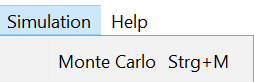
\includegraphics[width=4cm]{GUISimulation.png}
	\caption{Menuoption Simulation}
	\label{fig:GUISimulation}
\end{figure}	
\bigskip
		
\subsection{Graphische Anforderungen} \label{subsec:graphischeanforderungen}
In der Abbildung \ref{fig:GUI} ist der Aufbau der GUI ersichtlich.

\begin{figure}[H]
	\centering
	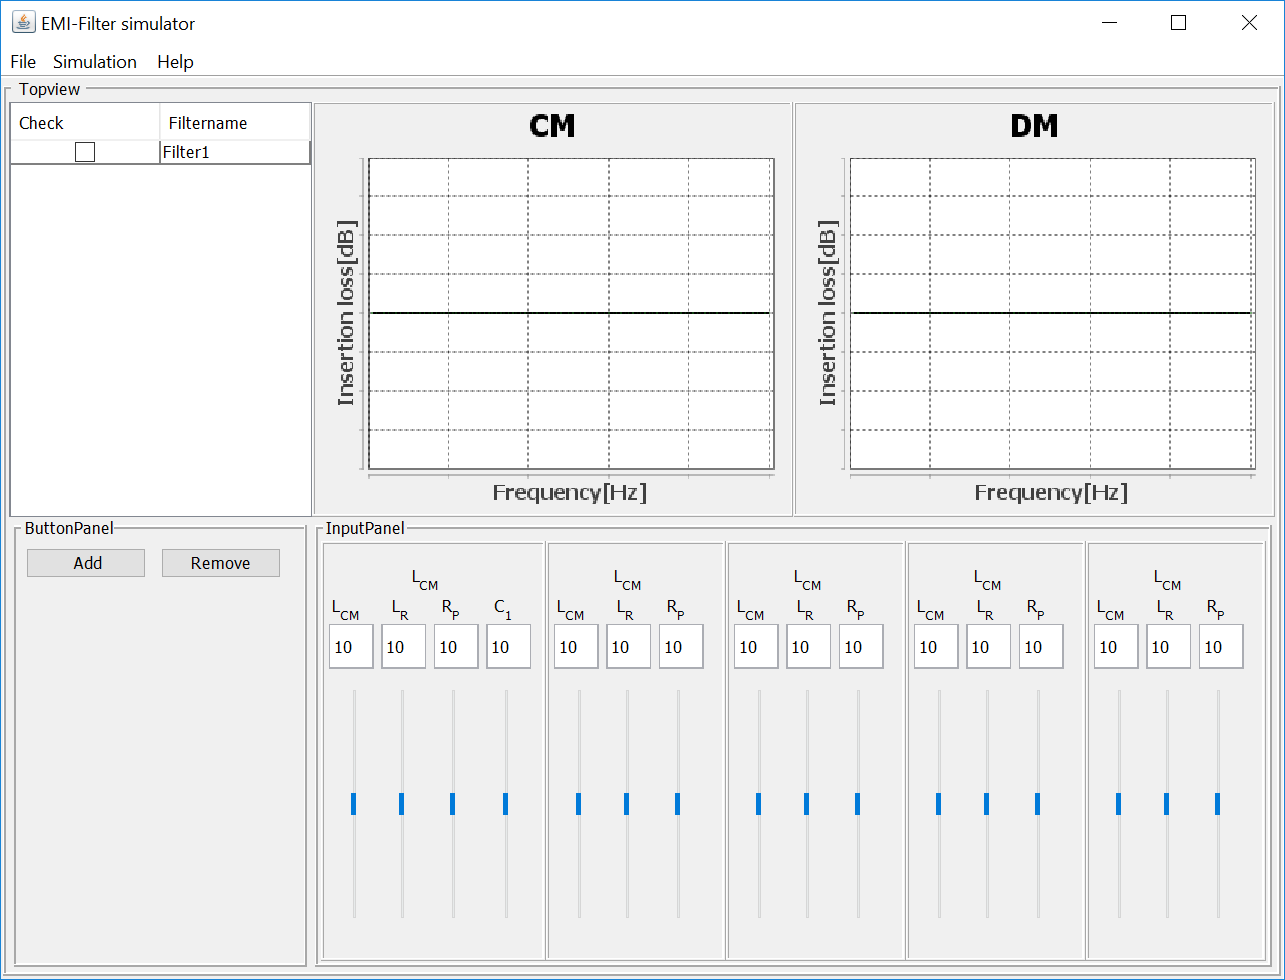
\includegraphics[width=10cm]{GUI.png}
	\caption{GUI}
	\label{fig:GUI}
\end{figure}

\bigskip
\subsubsection{Visualisierung der Schaltungen} \label{subsubsec:visualisierungderschaltungen}
Als generelle Hilfestellung soll das Programm dazu in der Lage sein, das elektronische Schema der jeweilig simulierten Schaltung anzuzeigen.
Im Menupunkt "Help" können die beiden CM- und DM äquivalenten Schaltungsmodelle, die zur Berechnung verwendet werden, in einem separaten Fenster dargestellt werden. Dieser Menupunkt ist in der Abbildung \ref{fig:GUIHelp} \nameref{fig:GUIHelp} dargestellt.

\begin{figure}[H]
	\centering
	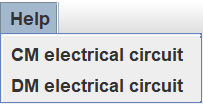
\includegraphics[width=4cm]{GUIHelp.png}
	\caption{Menuoption Help}
	\label{fig:GUIHelp}
\end{figure}
\shorthandon{"}
\bigskip

\subsubsection{Eingabemöglichkeiten}\label{subsubsec:eingabemöglichkeiten}
Da wir  die Auswirkungen hauptsächlich graphisch darstellen und analysieren wollen, und damit die Veränderungen nicht andauernd eingetippt werden müssen, greifen wir mithilfe eines Schiebereglers darauf zu. Das Eingabefenster (Abbildung: \ref{fig:GUIinputPanel}) ist dazu da, die einzelnen parasitären Filterparameter einzustellen und die Toleranz von ± 30\% mit einem Schieberegler zu variieren. Die Textfelder werden vor Fehleingaben geschützt indem sie  spezielle Eingabeformen (z.B. 10 milli=10m) unterstützen.
\begin{figure}[H]
	\centering
	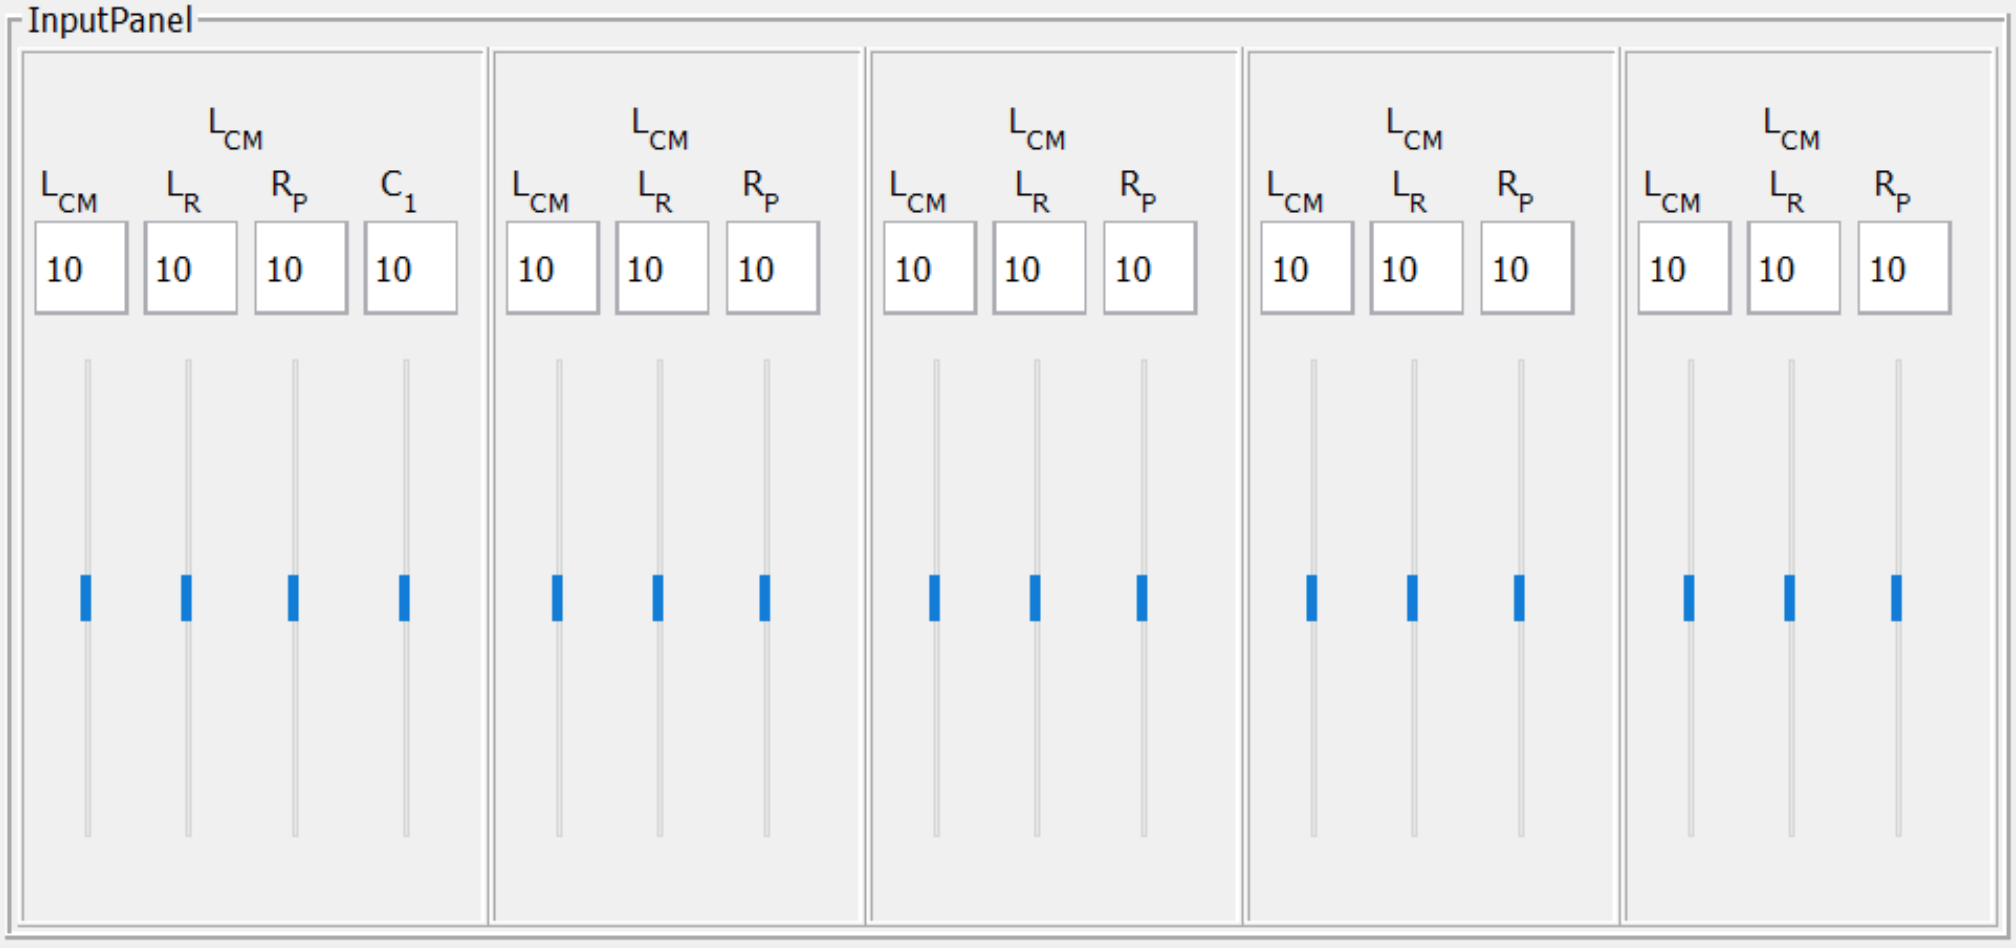
\includegraphics[width=10cm]{inputPanel.png}
	\caption{Eingabefenster}
	\label{fig:GUIinputPanel}
\end{figure}
\shorthandon{"}
\bigskip

\subsubsection{Mehrere Plots}\label{subsubsec:mehrereplots}
Das Programm hat seine Vorteile im direkten Vergleich von mehreren Simulationen. So können mehrere Filterprofile gleichzeitig im Plot angezeigt und verglichen werden. Die Abbildung \ref{fig:GUIplotPanel} stellt die Benutzeroberfläche für die beschriebene Anforderungen zur Verfügung.
\begin{figure}[H]
	\centering
	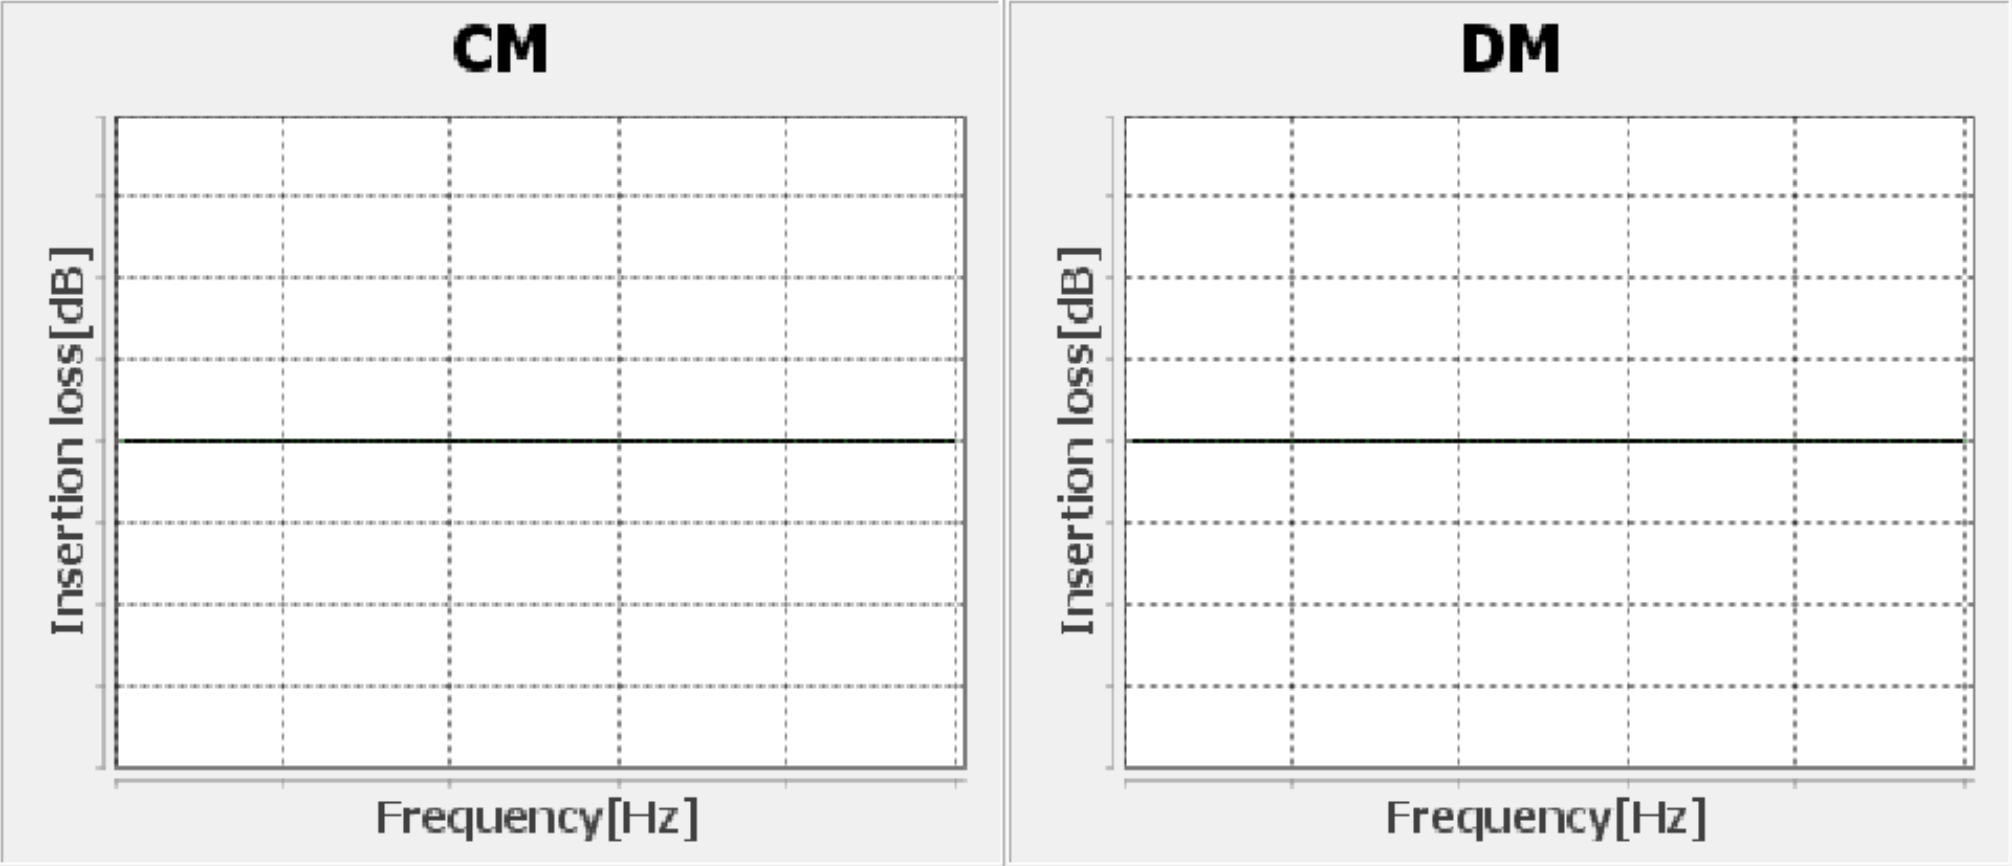
\includegraphics[width=12cm]{plotPanel.png}
	\caption{CM DM Plot}
	\label{fig:GUIplotPanel}
\end{figure}
\shorthandon{"}
\newpage
Im Fenster Abbildung \ref{fig:buttonPanel} können Filterprofile in die Filtertabelle geladen oder entfernt werden. Mit dem Button Add werden die eingegebenen parasitären Filterparameter in einem neuen Filterprofil gespeichert. Mit dem Button Remove wird das ausgewählte Filterprofil gelöscht.
\begin{figure}[H]
	\centering
	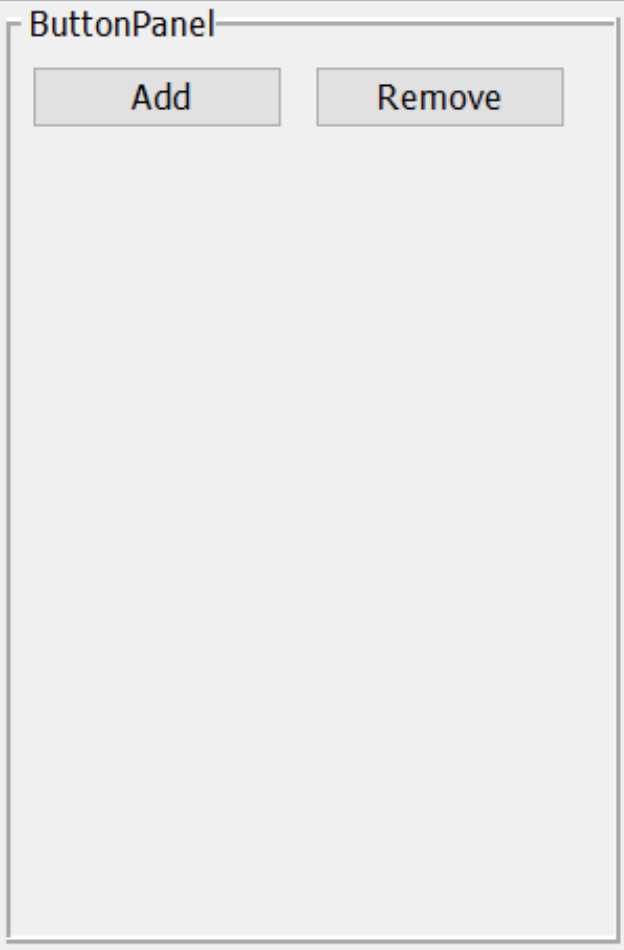
\includegraphics[width=4cm]{buttonPanel.png}
	\caption{Filterprofile}
	\label{fig:buttonPanel}
\end{figure}
\shorthandon{"}
\bigskip

\subsubsection{Frequenzbereich}\label{subsubsec:frequenzbereich}
Da das Frequenzspektrum sehr weit ist, werden die Plots logarithmisch zur Frequenzachse dargestellt. Sie werden farblich in 3 Bereiche unterteilt.
\bigskip
		
\subsection{Funktionelle Anforderungen} \label{subsec:funktionelleanforderungen}

\bigskip
\subsubsection{Speicherverwaltung}  \label{subsubsec:speicherverwaltung}
Um einen wirklichen Mehrwert zu schaffen soll die Software die Möglichkeit erhalten, eingestellte Filterprofile abzuspeichern und diese auch nach einem Neustart des Programms wieder zu verwenden. Im Menupunkt "File" können Filterprofile gespeichert und geladen werden. Bei beiden Optionen wird der Explorer geöffnet um die .txt Datei im gewählten Verzeichnis abzulegen oder zu holen. In der Option Exit kann das Programm geschlossen werden. Dieser Menupunkt ist in der Abbildung \ref{fig:GUIFile} \nameref{fig:GUIFile} dargestellt.
\begin{figure}[H]
	\centering
	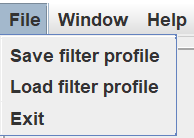
\includegraphics[width=4cm]{GUIFile.png}
	\caption{File}
	\label{fig:GUIFile}
\end{figure}
\shorthandon{"}
In der Filtertabelle Abbildung: \ref{fig:filterPanel} können alle erstellte Filterprofile dargestellt und verwaltet werden.  Mit einer Checkbox können einzelne Profile im Plot aus- bzw. eingeblendet werden. Zudem kann bei jedem Filterprofil ein Name hinzugefügt werden. Die Werte der parasitären Filterparameter des ausgewählten Filterprofils werden in das Eingabefenster geladen und können dort verändert werden. Mit den Shortcuts Backspace and Delete können ausgewählte Profile gelöscht werden.
\begin{figure}[H]
	\centering
	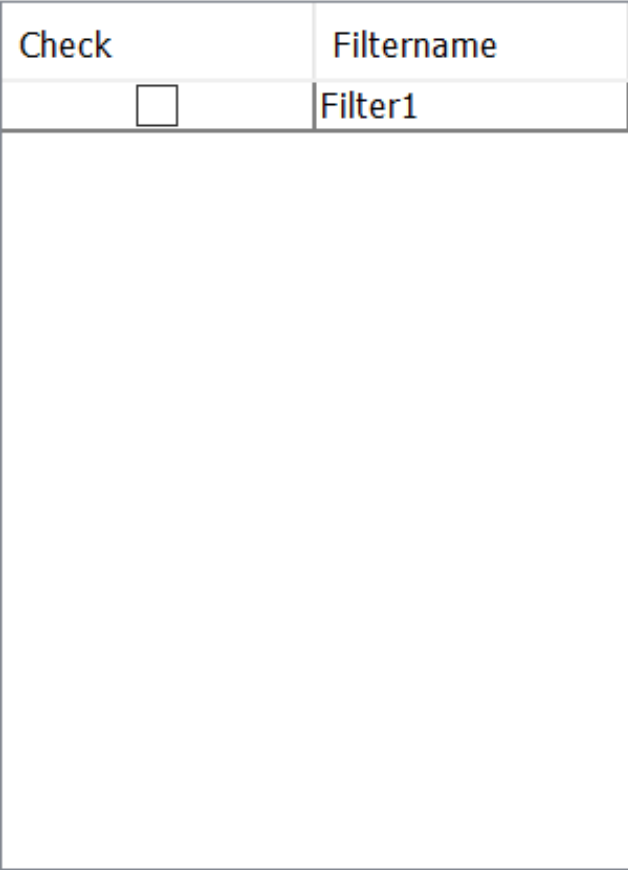
\includegraphics[width=4cm]{filterPanel.png}
	\caption{Filtertabelle}
	\label{fig:filterPanel}
\end{figure}
\bigskip

\subsubsection{Bedienungshilfen}\label{subsubsec:bedienungshilfen}
Um den User vor Fehleingaben zu schützen verwenden wir die von Herr Gut zur Verfügung gestellten Klassen.
Sämtliche Funktionen des Programms sind ebenfalls in einem Menu und mithilfe von Shortcuts aufrufbar.
Zudem können mit einem Rechtsklick auf den Plot verschiedene Optionen ausgewählt werden. So können die Eigenschaften (Farbe, Darstellung, Schrift usw.) und der Zoom individuell eingestellt werden. Ebenfalls soll es möglich sein die Plots als Bild zu exportieren um sie zu verwenden. Diese Optionen sind in der Abbildung \ref{fig:PlotSettings} ersichtlich.
\begin{figure}[H]
	\centering
	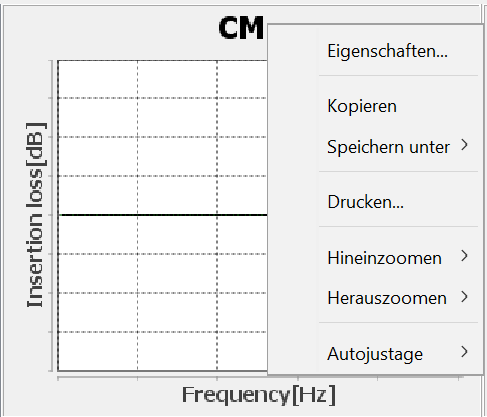
\includegraphics[width=4cm]{PlotSettings.png}
	\caption{Ploteinstellungen}
	\label{fig:PlotSettings}
\end{figure} 
\shorthandon{"}
\bigskip

\subsection{Libraries} \label{subsec:Libraries}

In der Software werden folgende Libraries verwendet:

\textbf{Swing}: Mit dem vorinstallierten Swing Framework von Java wird die GUI aufgebaut.\newline
\textbf{JFreeChart}: Die Berechnungen werden mit JFreeChart grafisch also Plot dargestellt. \cite{jfreechart} \newline
\textbf{Apache Math Commons}: Die Apache Math Commons Library beinhaltet wichtige Mathematikfunktionen, wie z.B. rechnen mit Komplexen Zahlen usw. \cite{apache}\newline
\textbf{Engineering Text Fields}: Die von Prof. Dr. Richard Gut zur Verfügung gestellte Klasse verhindert Fehleingaben und vereinfacht die Eingabe von Zahlen (nano,piko...)

\newpage

\section{Testkonzept}\label{sec:testkonzept}
Wieso, weshalb und Warum
\subsection{Prinzip} \label{prinzip}
Wie ist das Testkonzept aufgebaut
\subsection{Validierung} \label{validierung}
Testergebnisse darstellen und Interpretieren

Ebenfalls wird hier beschrieben welche Werte wir mit der Simulation und mit Matlab erreicht haben

\section{Projektvereinbarung} \label{sec:projektvereinbarung}
\begin{tabular}{l l}
\textbf{Auftraggeber} &\\
&\\
Dr. Luca Dalessandro \\
&\\
&\\
&\\
\rule{6cm}{0.5pt} & \rule{6cm}{0.5pt}\\
Ort, Datum & Unterschrift\\
&\\
&\\
&\\
&\\
&\\
&\\
\textbf{Projektleiter} &\\
&\\
Niklaus Schwegler&\\
&\\
&\\
&\\
\rule{6cm}{0.5pt} & \rule{6cm}{0.5pt}\\
Ort, Datum & Unterschrift\\
\end{tabular}



%%---BIBLIOGRAPHY------------------------------------------------------------------------

{\sloppypar
\selectlanguage{english}	
\setlength{\bibitemsep}{\baselineskip}
\printbibliography[heading=bibintoc]
\label{sec:lit}
}

%%---Anhang------------------------------------------------------------------------

\section{Anhang} \label{sec:anhang}



\subsection{Testkonzept} \label{subsec:eltech}
\begin{figure}[H]
	\centering
	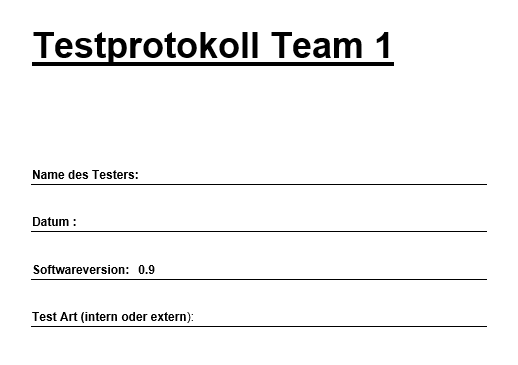
\includegraphics[width=16cm]{Protokoll.png}
	\label{fig:Protokoll}
\end{figure}

\begin{figure}[H]
	\centering
	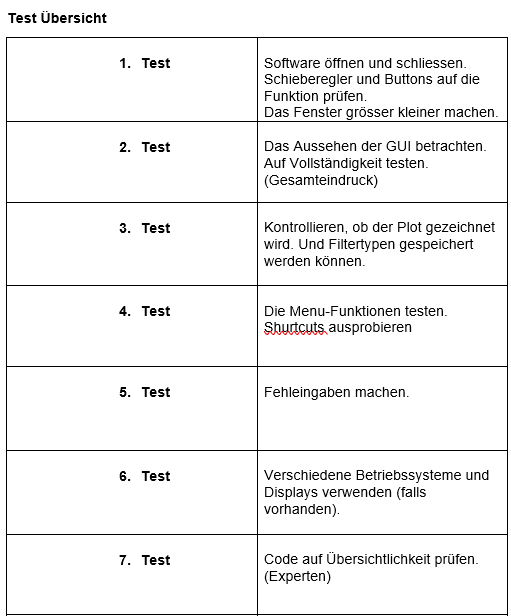
\includegraphics[width=16cm]{uebersicht.png}
	\label{fig:übersicht}
\end{figure}

\begin{figure}[H]
	\centering
	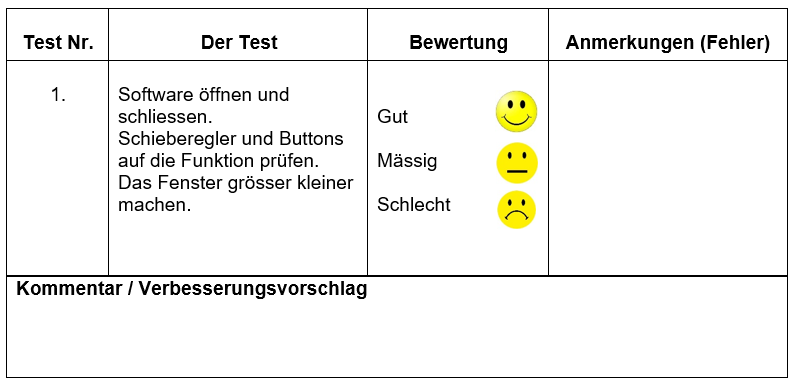
\includegraphics[width=16cm]{Test1.png}
	\label{fig:Test1}
\end{figure}

\begin{figure}[H]
	\centering
	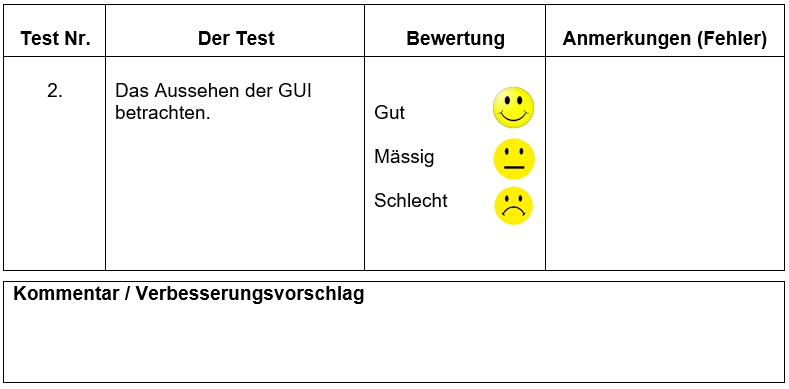
\includegraphics[width=16cm]{Test2.png}
	\label{fig:Test2}
\end{figure}

\begin{figure}[H]
	\centering
	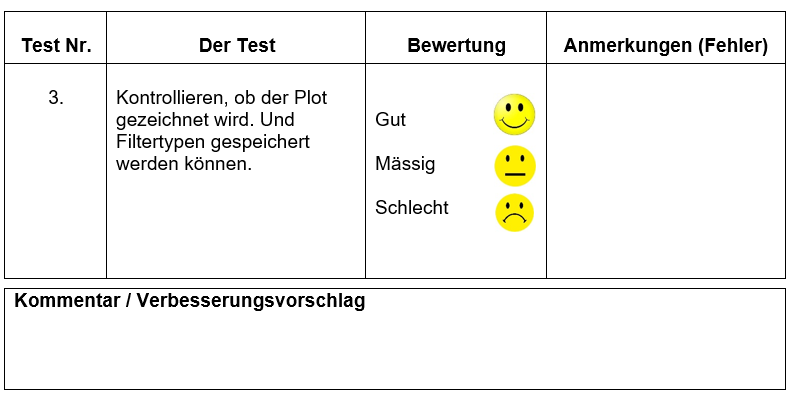
\includegraphics[width=16cm]{Test3.png}
	\label{fig:Test3}
\end{figure}

\begin{figure}[H]
	\centering
	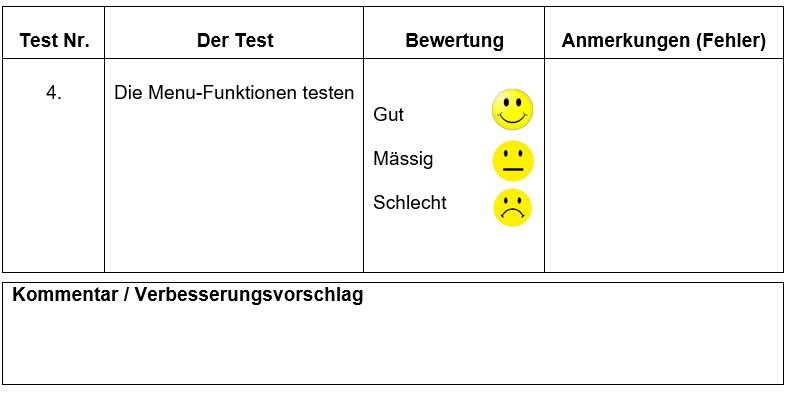
\includegraphics[width=16cm]{Test4.png}
	\label{fig:Test4}
\end{figure}

\begin{figure}[H]
	\centering
	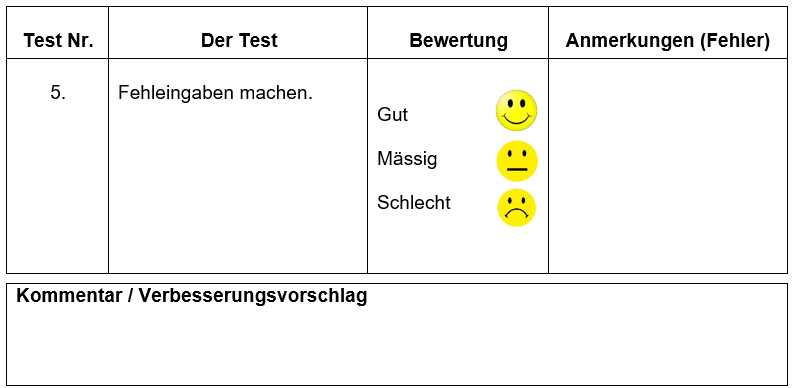
\includegraphics[width=16cm]{Test5.png}
	\label{fig:Test5}
\end{figure}

\begin{figure}[H]
	\centering
	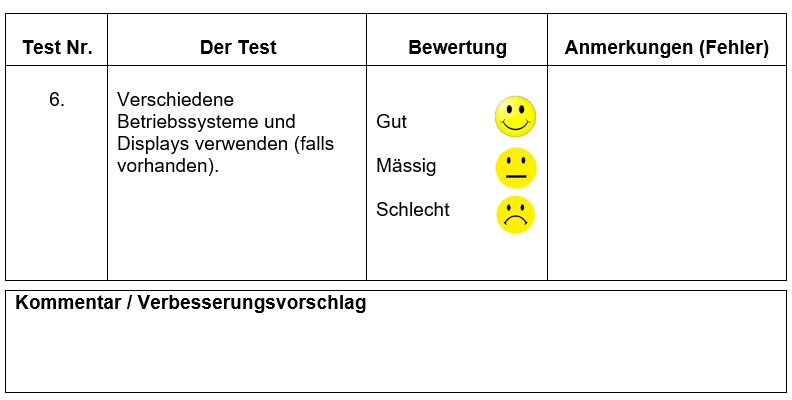
\includegraphics[width=16cm]{Test6.png}
	\label{fig:Test6}
\end{figure}

\begin{figure}[H]
	\centering
	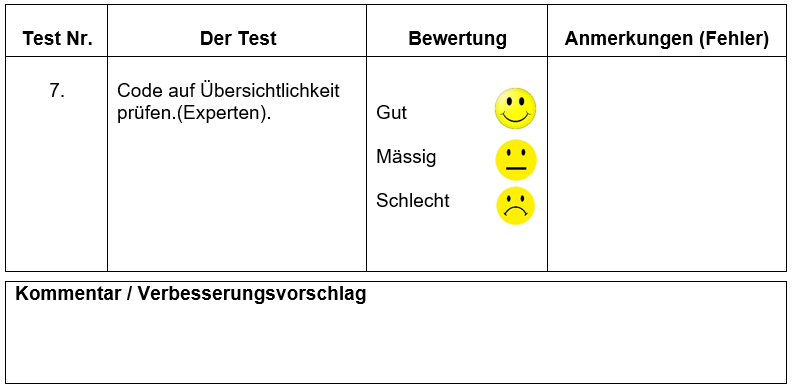
\includegraphics[width=16cm]{Test7.png}
	\label{fig:Test7}
\end{figure}

\begin{figure}[H]
	\centering
	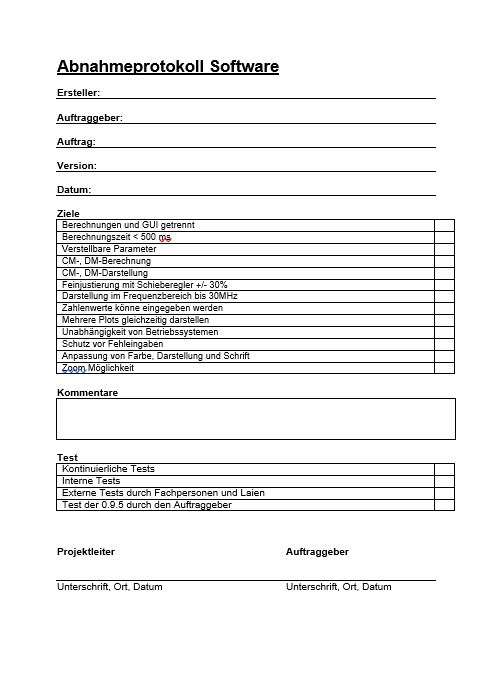
\includegraphics[width=16cm]{Abnahme.png}
	\label{fig:Protokoll}
\end{figure}

%%---NOTES for DEBUG---------------------------------------------------------------------
\ifdraft{%Do this only if mode=draft
%%requires \usepackage{todonotes})
\newpage
\listoftodos[\section{Todo-Notes}]
\clearpage
}
{%Do this only if mode=final
}
\end{document}
